\documentclass[a5paper,9pt]{scrartcl}
\usepackage{nameref}
\usepackage[hyphens]{url}
\usepackage{hyperref}
\usepackage[utf8]{inputenc}
\usepackage{menukeys}
\usepackage{listings}
\usepackage{hyperref}
\usepackage{framed}
\usepackage{graphicx}
\usepackage{float}

\newcommand*{\mybox}[1]{\framebox{#1}}

\title{Windows workflow}

%Vinkkejä koneella työskentelyn nopeuttamiseksi

\begin{document}
	
	\maketitle
	
	\tableofcontents
	
	\newpage
	
    \section{Johdanto}\label{Johdanto}
    Tässä dokumentissa käydään läpi erilaisia tapoja helpottaa ja nopeuttaa tutkijan työskentelyä. Aluksi käymme läpi yksinkertaisia, tietokoneen sisään rakennettuja ominaisuuksia, jonka jälkeen siirrymme monimutkaisempiin ongelmiin.
    
    \section{Peruspikanäppäimet}
    \label{perus}
    
    Lämmitellään ensin peruspikanäppäimillä, jotka toimivat ilman kaikilla windows-koneilla, ilman Autohotkeyta.
    
    \subsection{Windows}
    
    
    \indent 
    
    \keys{Win}+\keys{"kirjoita ohjelman X nimi"}+\keys{\return} Avaa ohjelma X ilman hiirtä
    
    \keys{Win}+ [ \keys{\arrowkeyleft} \keys{\arrowkeyright} \keys{\arrowkeyup} \keys{\arrowkeydown} ] siirrä ikkunoita. 
    
    \keys{Ctrl}+\keys{F} Etsi sivulta tekstiä

    
    \keys{Ctrl}+\keys{C} Kopioi 
    
    \keys{Ctrl}+\keys{V} Liitä 
    
    \keys{Ctrl}+\keys{\shift}+\keys{V} Liitä ilman muotoilua
    
    \keys{Ctrl}+\keys{X} Leikkaa 
    
    \keys{Ctrl}+\keys{A} Valitse kaikki
    
    \keys{Ctrl}+\keys{Z} Kumoa
    
    \keys{Ctrl}+\keys{Y} tai..
    
    \keys{Ctrl}+\keys{Shift}+\keys{Z}  Vastatoiminto kumoamiselle (vaihtelee ohjelmittain)
    
    \keys{Alt}+\keys{Tab} Vaihtele kahden viimeisimmän ikkunan välillä
    
    \keys{Alt}+\keys{Tab}+\keys{Tab}+\keys{Tab}...vaihtele kaikkia käynnissä olevia ikkunoita
    
    \subsection{Firefox/Chrome}
    
    \indent
    
    \keys{Ctrl}+\keys{L} kirjoita verkko-osoite tai goolge-haku ilman hiirtä
    
    \keys{Ctrl}+\keys{Tab} mene seuraavaan välilehteen
    
    \keys{Ctrl}+\keys{T} Uusi välilehti
    
    \keys{Ctrl}+\keys{W} Sulje välilehti
    
    \keys{Ctrl}+\keys{Shift}+\keys{T} Palauta (vahingossa) suljettu välilehti

    
    
    %\keys{Ctrl}+\keys{1} mene 1. välilehteen (toimii vastaavasti muilla numeroilla)
	\url{https://support.mozilla.org/en-US/kb/keyboard-shortcuts-perform-firefox-tasks-quickly}
	
	
	%testing:
	%\expandafter\def\expandafter\UrlBreaks\expandafter{https://support.mozilla.org/en-US/kb/keyboard-shortcuts%
	%	-perform-firefox-tasks-quickly}
	

    
    \url{https://support.google.com/chrome/answer/157179?hl=en}
    
    
	\subsection{Outlook}
	
	\indent
	
	\keys{\ctrl + 2} Kalenteri
	
	\keys{\ctrl + 1} Sähköposti
	
	\keys{\ctrl + ,} edellinen viesti
	
	\keys{\ctrl + .} seuraava viesti
	
	\keys{\ctrl + N} Uusi viesti
	
	\keys{\ctrl + R} Vastaa
	
	\keys{\ctrl + F} Välitä eteenpäin
	
	\keys{\ctrl + \return} Lähetä
	
	\medskip
	
		Lisää viestipohja (Quick parts) uutta viestiä kirjoittaessasi ks. kuva \ref{fig:Quick_parts}  niin vältät kirjoittamasta samoja asioita toistamiseen.
		
		\menu{Insert>Quick Parts}
		
		\menu{Lisää>Pikaosat} tms.
		
		 Sen jälkeen saat viestipohjan käyttöön uutta viestiä kirjoittaessa painamalla \\ \keys{Alt}+\keys{N}+\keys{Q}+\keys{\return}
	 
	\begin{figure}[H]
		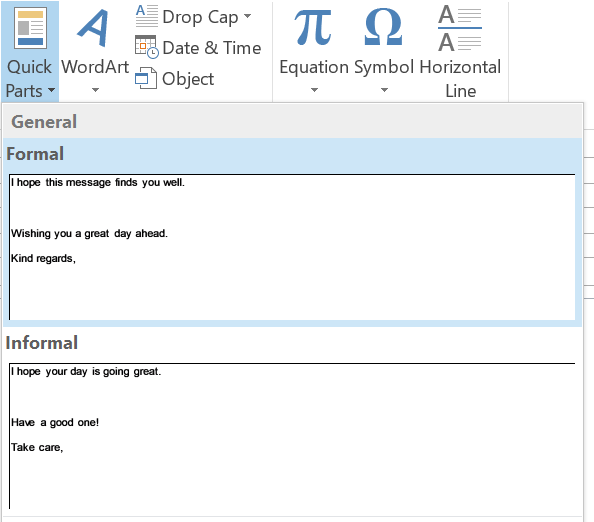
\includegraphics[width=\linewidth]{Quick_parts.png}
		\caption{Esimerkkejä Outlookin viestipohjista (Quick parts)}
		\label{fig:Quick_parts}
	\end{figure}

	\medskip
	
	Lisää Outlookin pikanäppäimiä: \url{https://support.office.com/en-us/article/keyboard-shortcuts-for-outlook-3cdeb221-7ae5-4c1d-8c1d-9e63216c1efd}
	
	\subsection{Youtube}
	
	\indent
	
	\keys{\shift + .} Nopeuta videota
	
	\keys{\shift + ,} Hidasta videota
	
	\keys{F} Koko ruudun tila
	
	\keys{\keys{\arrowkeyright}} tai \keys{L} Mene 5/10 sekuntia eteenpäin
	
	\keys{\keys{\arrowkeyleft}} tai \keys{J} Mene 5/10 sekuntia taaksepäin
	
	\url{https://youtu.be/UlB7TJ6cTx4}
    
    \pagebreak \section{Ladattavat ohjelmat ja koodi}
    Osiota \ref{perus} \nameref{perus} lukuunottamatta tarvitset seuraavat ohjelmat ja koodin.
    
    \subsection{Zotero}
    \url{https://www.zotero.org/download/}
    
    
    Lataa sekä ''Zotero for Windows'', että ''Zotero Connector''. Tämän jälkeen viitteet saat tallennettua Firefoxissa/Chromessa painamalla hiirellä selaimen oikeaa yläkulmaa (edellyttäen, että Zotero-sovellus on auki).
    
    \subsection{Autohotkey}
    \url{https://www.autohotkey.com/download/}
    Valitse ''Download Autohotkey Installer''
    
    \subsubsection{Autohotkey scriptit} \label{downloads}
   
    \begin{framed}
   
   \underline{1.Mene osoitteeseen:}
   
   \url{https://github.com/samuelsaari/workflow})
   
   \medskip
   
   \underline{2. Lataa tiedostot}
    
    windows\_workflow.ahk
    
    stata\_workflow\_A.ahk
    
    stata\_workflow\_B.ahk
    
    word\_macros.txt
    
    \medskip
    
    \underline{3.Lataa myös tiedostot kansiosta Useful\_material}
    
   
    Erityisesti \textbf{shorcut\_chart.pdf} on hyvä katsoa läpi, koska siinä näkyy suhteellisen havainnollisesti suurin osa autohotkey-pikanäppäimistä. Muita tiedostoja Useful\_material-kansiosta et välttämättä tarvitse akuutisti, mutta niille tulee luultavasti käyttöä jossain vaiheessa, joten ne on hyvä ladata valmiiksi.
    
    \end{framed}

    
    \medskip
  
     Ahk-scriptit aktivoituvat tuplaklikkaamalla. Jotta scripti pyörii myös sen jälkeen, kun olet käynnistänyt tietokoneen uudestaan, luo tiedostosta pikakuvake ja laita se windowsin käynnistys-kansioon.
    
    \medskip
    
    \emph{WINDOWS 10}: Paina \keys{Win}+\keys{r} ja kirjoita ilmestyvään ruutuun \mybox{shell::startup} ja paina \keys{\return}. Tämän jälkeen Copy-pastaa luomasi pikakuvake aloituskansioon
    
    \medskip
    
    \emph{WINDOWS 7}: Paina \keys{Win}+\keys{r} ja kirjoita ilmestyvään ruutuun 
    
    \emph{C:/users/\textbf{*YOURUSERNAME*}/AppData/Roaming/Microsoft/Windows/Start Menu/Programs/Startup} 
    
    ja paina \keys{\return}. *YOUR USERNAME* korvataan siis sinun käyttäjätunnuksellasi, esim. mmak (sama millä kirjaudutaan windowsiin ja Outlook webiin)
    Tämän jälkeen Copy-pastaa luomasi pikakuvake aloituskansioon.
    
    
    \subsection{Word}
    Word on luultavasti sinulla  jo valmiiksi asennettuna, mutta tarvitset koodinpätkän, jotta seuraavat jutut toimivat. Kun word on auki paina \keys{Alt}+\keys{F11} ja Copy-pastaa (\keys{Ctrl}+\keys{c} \& \keys{Ctrl}+\keys{v}) tiedostossa \textbf{word\_macros.txt} oleva koodi käytettävissä olevaan isoon tilaan. Tiedosto löytyy \href{https://github.com/samuelsaari/workflow}{Githubista}, ks. osio \ref{downloads}. Tallenna macrot (\keys{Ctrl}+\keys{s}) ja palaa Wordin perunäkymään.
    
    Tämän jälkeen on vielä alustettava pikanäppäimet ennen ensimmäistä käyttöä:
    
    \menu{Näytä > Makrot > Näytä makrot} 
    
    \menu{View > Macros > View Macros} ja aja kaikki "SC" päätteiset makrot.
    
    Lopuksi käynnistä word uudelleen. 
    
    %\begin{lstlisting}[frame=single]
    %\end{lstlisting}
    
    
    \section{Autohotkey pikanäppäimet Windosille ja Statalle}
    Valtaosa pikanäppäimistä löytyy kätevästi tiedostosta \textbf{shorcut\_chart.pdf} kansiosta \emph{Useful\_material} linkin \url{https://github.com/samuelsaari/workflow} takaa.
    
    \subsection{Ohjelmien käynnistäminen ja niiden välillä liikkuminen}
    
     Suurin osa pikanäppäimistä avaa/aktivoi ohjelman tai ikkunan, mutta myös joitain usein toistuvia toimia on automatisoitu.
    
    \medskip
    
    Alla eritelty joitain esimerkkejä pikanäppäimistä.
    
    Yleisesti \keys{Alt}+\keys{"näppäin"} tekee kullekin ohjelmalle jotain seuraavista:
    
    - Jos ohjelma ei ole auki, avaa ohjelma
    
    - Jos ohjelmasta on yksi ikkuna auki, ikkuna minimoidaan
    
    - Jos ohjelmasta on yksi ikkuna käynnissä, mutta ei näy näytöllä, se saadaan näkyviin
    
    - Jos ohjelmasta on useampi ikkuna käynnissä, pikanäppäin kierrättää näitä ikkunoita
    
    \medskip
    
    \keys{Alt}+\keys{A} esimerkiksi avaa, minimoi/maksimoi tai kierrättää kansioita.
    
     \keys{Alt}+\keys{CapsLock} taas avaa, minimoi/maksimoi tai kierrättää firefox-ikkunoita.
    
    
    \keys{Alt}+\keys{S} "Ota screenshot" on erityisen hyödyllinen. (Vain Win10, kaikki päivitykset tehtynä)
    
    
      
    \subsection{Viitteet}
    
    \subsubsection{Viitteiden lisääminen Zoteroon Firefoxissa}
    \keys{\ctrl + \shift + S}
    
    Tämä toimii jossain määrin myös ilman Autohotkeytä, mutta tällä lailla viitteet tallentuvat pdf-tiedostoineen varmemmin.
    
    \subsubsection{Lähdeviittaaminen Wordissa}
    
    \keys{\ctrl + å}
    Tämä pikakomento tekee monta asiaa, riippuen tilanteesta:
    
    - lisää uuden viitteen
    
    - muokkaa olemassa olevaa viitettä
    
    - poistaa kirjoittajan (2019) viittauksesta
    
    - Palauttaa kirjoittajan viitteeseen (Saari, 2019). Siis edellisen käänteistoiminto
    
    - avaa viittausikkunan, jos se on olemassa, mutta ei ole aktiivinen
    
    
    Lisäksi on hyvä tietää, että kaksoispisteen \keys{:} avulla viitteen perään saa sivunumerot.
    
    Kun dokumentti on valmis, lisää lähdeluettelo wordiin pikanäppäimellä:
    
    \keys{\ctrl}+\keys{Alt}+\keys{B}
    
    Olemassa olevan lähdeluettelon päivitys:
    
    \keys{\ctrl + \shift+ å}
    
    Näin välttyy kokonaan viitteiden tarkistamiselta, ja monelta muulta harmilta.
    
    \subsubsection{Lähdeviitteiden tarkistaminen Wordissa (extra)}
    Käytettyjen lähdeviitteiden tarkistaminen onnistuu kätevästi jakamalla ruutu kahtia.
    
    \menu{Näytä > (Järjestä) > Jaa }
    
    \menu{View > (Arrange) > New Window}
    
    Ks. lisätiedot:
    
    \url{https://support.office.com/en-us/article/view-two-parts-of-a-document-at-the-same-time-in-word-for-mac-1adf3317-0ec4-4568-ad32-6f68b3e4b386}
    
    Tämän jälkeen lue teksti alusta loppuun ja merkitse käytetyt viitteet värittämällä ne. Yhden lähdeviitteen (kappaleen) korostaminen onnistuu pikakomennolla
    
    \keys{Ctrl}+\keys{ö}. 
    
    Jos haluat poistaa värityksen yhdestä viitteestä (kappaleesta) paina
    
    \keys{ctrl}+\keys{ä}
    
    Kun olet päässyt tekstin loppuun, voit poistaa värjäämättömät viitteet, poistaa värit ja dokumentin kahtia jaon. Jos käytät Zoteroa niin tällaista tarkistustahan ei tarvi tehdä!
    
    \subsection{Stata}
    
    Ks. \textbf{shorcut\_chart.pdf}, alla muutama esimerkki.
    
    \medskip
    
    \keys{Win}+\keys{CapsLock} Stata pääikkuna
    
    \keys{Win}+\keys{\shift} Do-file
    
    \keys{Win}+\keys{\textgreater} Ensin Stata, Sitten do-file
    
    \keys{Win}+\keys{Q} Editor
    
    \keys{Win}+\keys{A} Graph
    
    \keys{Win}+\keys{Z} Viewer
    
    \medskip
    
    \keys{\ctrl}+\keys{D} Aja koko do-file
    
    \keys{\ctrl + \return} Aja rivi koodia
    
    \keys{Alt}+\keys{\return} Aja koodia merkkien \keys{\{} \keys{\}} välissä
    
    \keys{Ctrl}+\keys{Alt}+\keys{B} Aja do-file siihen asti, missä tekstikursori on
    
    
%   \section{Extra}
%    You can visualize paths \directory{/home/moose/Desktop/manual.tex}
%    or menus \menu{View > Highlight Mode > Markup > LaTeX} or key
%    press combinations: \keys{\ctrl + \shift + F} is for formatting
%    in Eclipse.
%    You can also visualize \keys{\tab}, \keys{\capslock}, \keys{\Space}, 
%    \keys{\arrowkeyup} and many more.
%    Let's try some more: \keys{a}, \keys{ä} 

    
\end{document}